%%%%%%%%%%%%%%%%%%%%%%%% HAUB.tex %%%%%%%%%%%%%%%%%%%%%%%
%
% Root file for: Moving Mars (D. Hyland-Wood) November 2016
%
%%%%%%%%%%%%%%%%%%%%%%%%%%%%%%%%%%%%%%%%%%%%%%%%%%%%

%\documentclass[10pt]{book} % 10 point font
%\documentclass[11pt]{book} % 11 point font
\documentclass[12pt]{book} % 12 point font
\usepackage[a4paper, top=3cm, bottom=3cm]{geometry}
\usepackage[utf8]{inputenc}
%\usepackage[latin1]{inputenc}
\usepackage{setspace}
\usepackage{fancyhdr}
\usepackage{tocloft}

% Extension Packages
%-------------------------------------------------------------------------------
\usepackage{mathptmx}	% selects Times Roman as basic font
\usepackage{helvet}		% selects Helvetica as sans-serif font
\usepackage{courier}	% selects Courier as typewriter font
%\usepackage{type1cm}	% activate if the above 3 fonts are 
					% not available on your system
					
\usepackage{titling}
\newcommand{\subtitle}[1]{%
  \posttitle{%
    \par\end{center}
    \begin{center}\large#1\end{center}
    \vskip0.5em}%
}

\newenvironment{dedication}
    {\vspace{6ex}\begin{quotation}\begin{center}\begin{em}}
    {\par\end{em}\end{center}\end{quotation}}
    
\usepackage{makeidx}	% allows index generation
\usepackage{graphicx}	% standard LaTeX graphics tool
					% when including figure files
\usepackage{multicol}	% used for the two-column index
\usepackage[bottom]{footmisc}% places footnotes at page bottom

%\usepackage{url}		% Avoid problems with special characters in URLs
\PassOptionsToPackage{hyphens}{url}
\usepackage{hyperref}
\usepackage{breakurl}	% Apparently cannot be used when processing with pdflatex.

\usepackage{soul}		% Allow line breaks in underlined text.

\usepackage{listings}
\lstset{basicstyle=\small, columns=fixed}

\usepackage{amsmath}

% Fix hyphenation
\tolerance=700
\setlength{\emergencystretch}{3em}

% For layout of poetry
\usepackage{lettrine}
\usepackage{parselines}
\usepackage{xcolor}
%\definecolorseries{verso}{rgb}{last}{blue!40!black}{magenta!40!black}
\definecolorseries{verso}{rgb}{last}{black}{black}
\resetcolorseries[30]{verso}
\newenvironment{verso}{\pagebreak[3]\begin{parse lines}[\parindent=1em\noindent]{\color{verso!!+}\hspace{\row\parindent}##1\newline\color{black}}}%
{\end{parse lines}}

%\usepackage{tocbibind}	% Allows the bibliography to appear in the TOC.

\makeindex			% used for the subject index
					% NB: Springer uses the style svind.ist with the makeindex program. 
					% TODO: Should I?

% Use a single bibliography style
%\usepackage[super]{natbib} % Makes citations superscript, which is nicer but conflicts with footnotes. TODO: Change somehow.
\bibliographystyle{plain}

% Custom
%-------------------------------------------------------------------------------
%\usepackage{cyrillic}
\usepackage[T1]{fontenc}   % Allows words with accented characters to be cut-and-pasted, and hyphenated.
\usepackage{enumitem}
\usepackage{phonetic}

% For title page
\newcommand{\HRule}{\rule{\linewidth}{0.5mm}}
\usepackage[export]{adjustbox}

% For Russian (Cyrillic) names in endnotes:
%\newcommand{\cyrrm}{\fontencoding{OT2}\selectfont\textcyrup} % cyrrm = "Roman", or really upright, normal font

\lstset{
      basicstyle = \scriptsize \ttfamily,%
      keywordstyle = [1]\bfseries\color{darkgreen},%
      stringstyle  = \ttfamily\color{darkred},%
      commentstyle = \itshape\color{darkblue},%
      showstringspaces = false,%
%     fancyvrb = true,%
      firstnumber = auto, stepnumber=1, numbersep=5pt,%
      numbers=left, numberstyle=\tiny \ttfamily,
      frame = shadowbox, frameround = ffff, rulesepcolor = \color{shadecolor},
      breaklines=true, breakatwhitespace=true,%
%      prebreak=\textellipsis,postbreak=\textellipsis,%
      emphstyle = \color{red}\underbar, emphstyle = {[2]\color{blue}\underbar},%
      extendedchars = true, inputencoding = utf8,%
%     backgroundcolor=\color{shadecolor},
      xleftmargin=5pt, xrightmargin=2pt,
      captionpos = b
}

\usepackage{eso-pic}
\newcommand\BackgroundPic{%
\put(0,0){%
\parbox[b][\paperheight]{\paperwidth}{%
\vfill
\centering
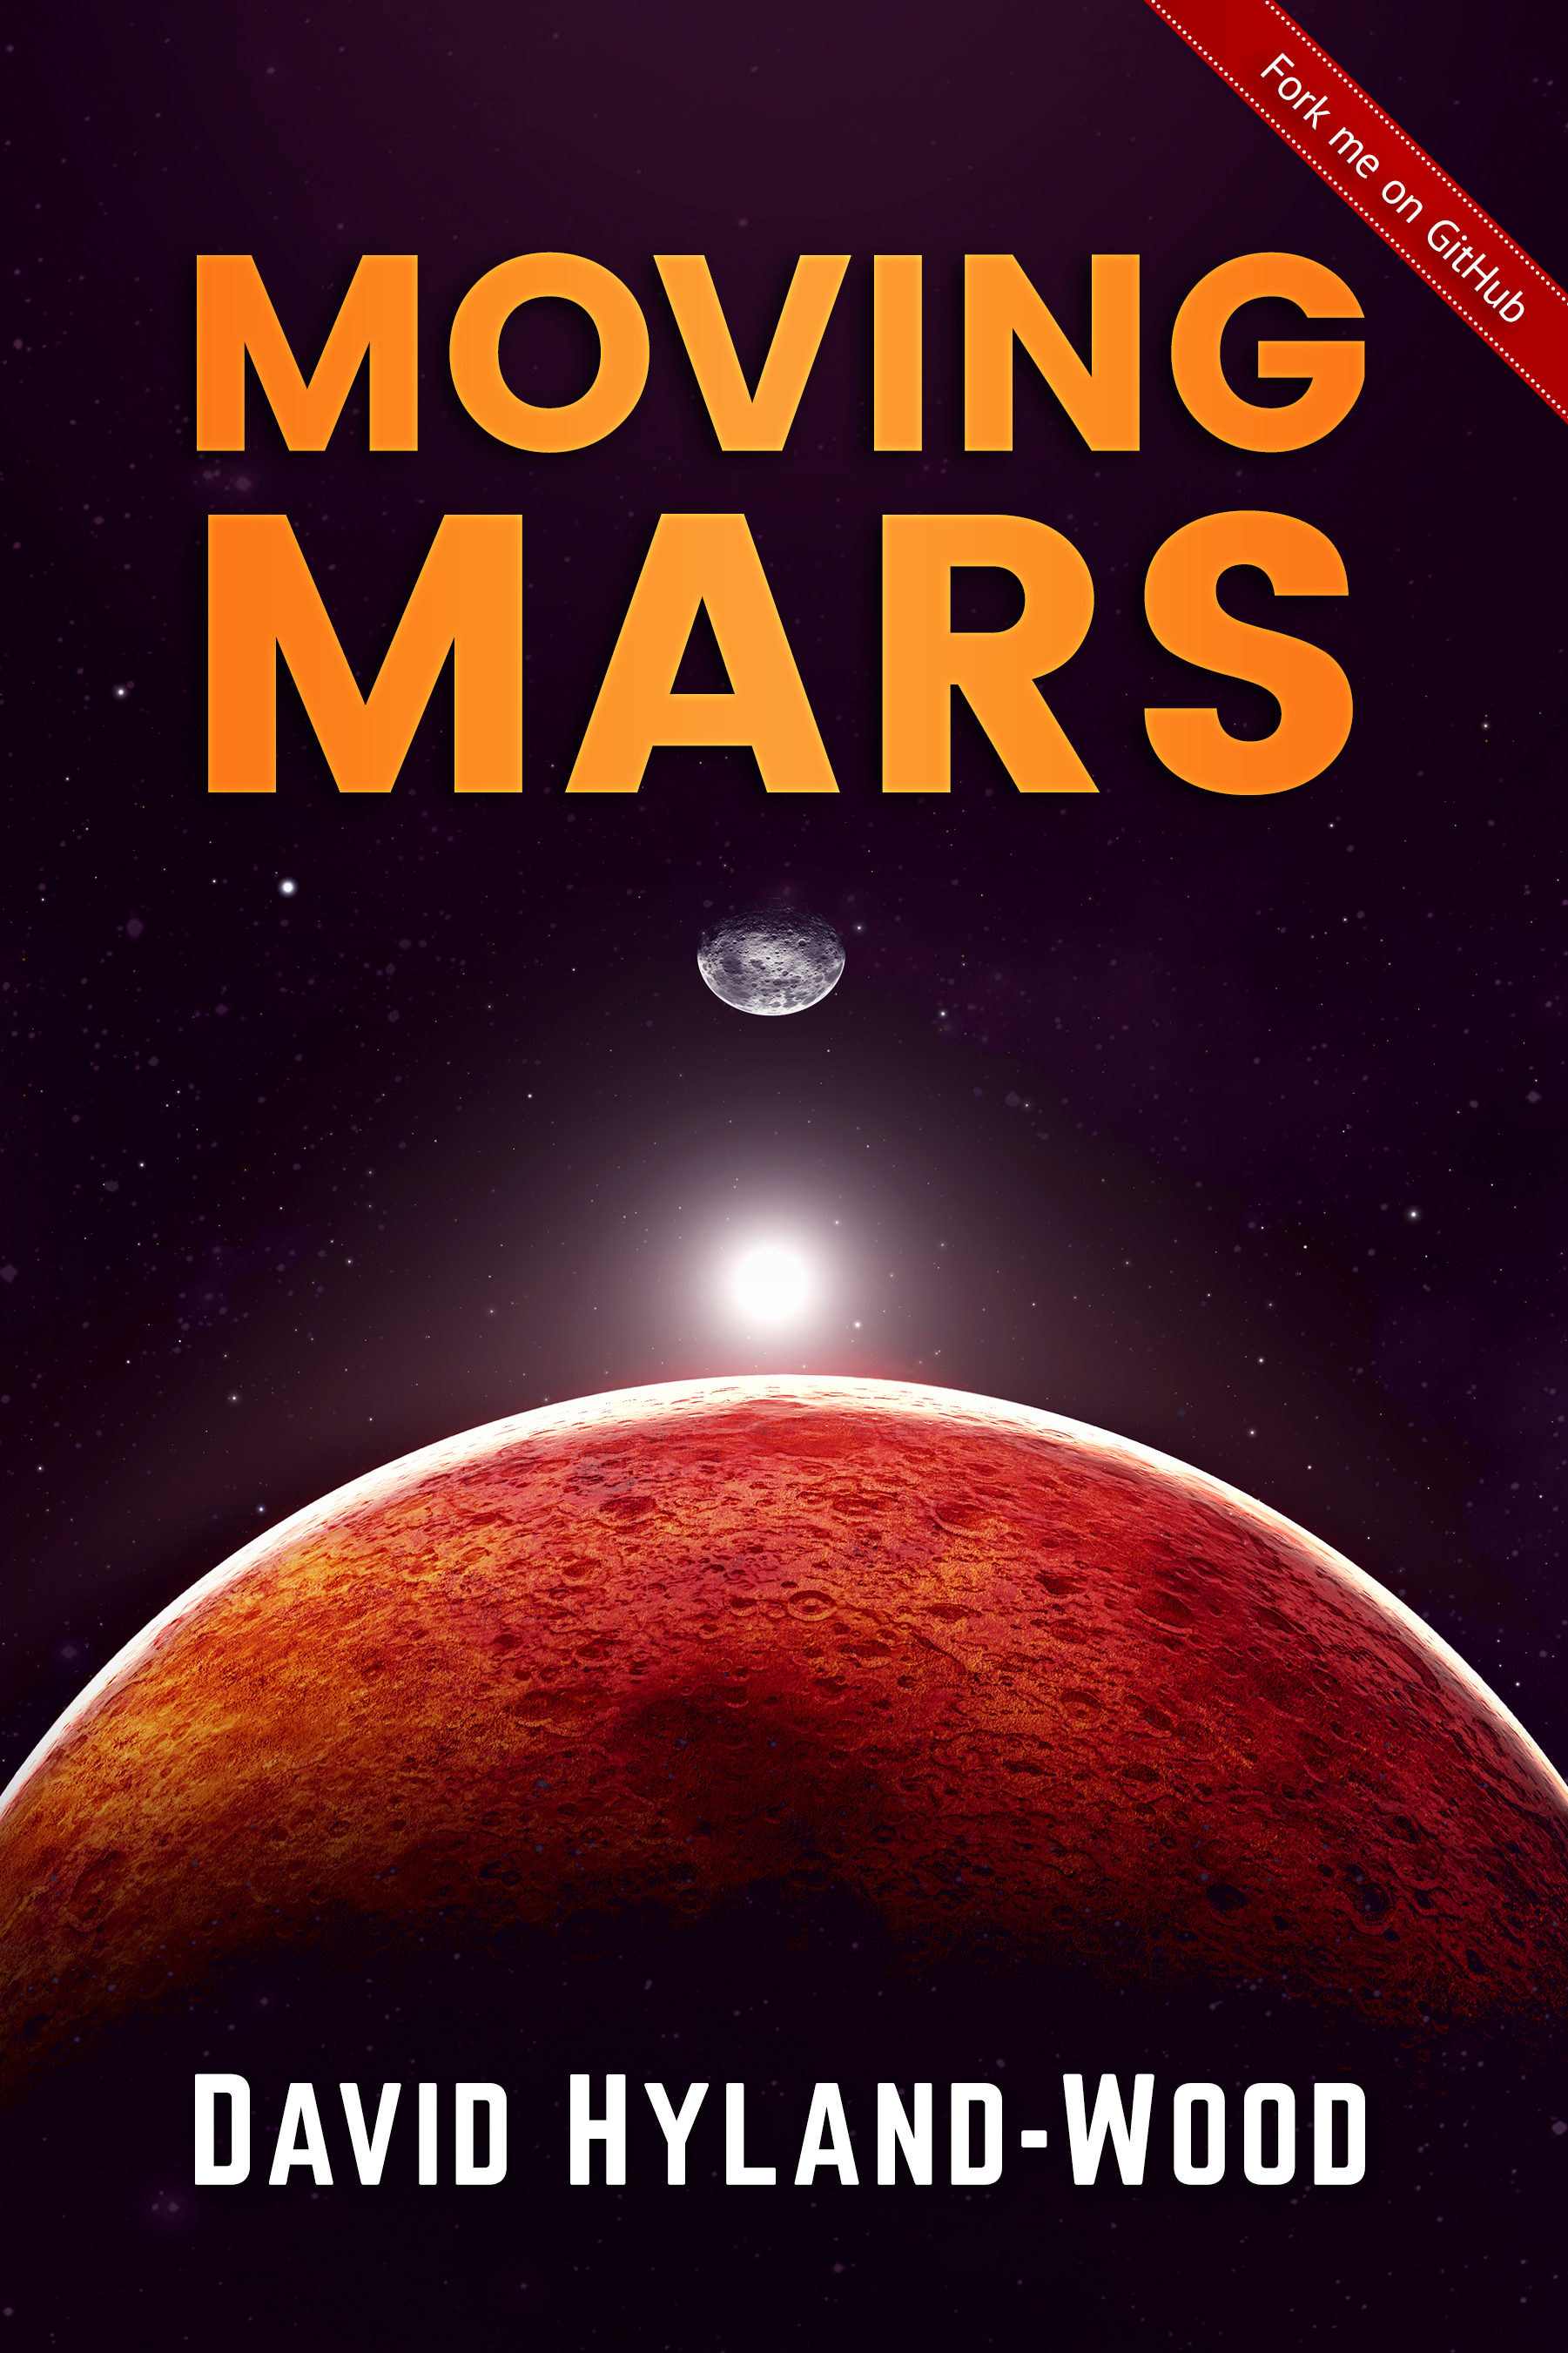
\includegraphics[width=\paperwidth,height=\paperheight,%
keepaspectratio]{cover/MovingMarsfront.jpg}%
\vfill
}}}
% End Custom
%-------------------------------------------------------------------------------

\begin{document}


% Graphical Cover
%-------------------------------------------------------------------------------
\AddToShipoutPicture*{\BackgroundPic}
\newpage
\thispagestyle{empty}
\mbox{}
\newpage

% Title Pages
%-------------------------------------------------------------------------------
\pagestyle{empty}

\begin{titlepage}

\vspace*{\fill}
\noindent
\textsc{Preview Edition, \today}

\vspace{5 mm}
\noindent
Moving Mars by David P. Hyland-Wood, published by David P. Hyland-Wood, PO Box 4028, St Lucia South 4067 QLD Australia

\vspace{5 mm}
\noindent
www.hyland-wood.org

\vspace{5 mm}
\noindent
Copyright \textcopyright { }2021 by David P. Hyland-Wood

\vspace{5 mm}
\noindent
Permission is granted to copy, distribute and/or modify this document
under the terms of the GNU Free Documentation License, Version 1.3
or any later version published by the Free Software Foundation;
with the Invariant Sections being  "Acknowledgements", "Dedication",
and "History", no Front-Cover Texts, and no Back-Cover Texts.
For additional permission requests, write to the publisher, using ``Attention: Permissions Coordinator,'' at books@hyland-wood.org.

\vspace{5 mm}
\noindent
This is a work of fiction. Names, characters, places, and incidents either are the products of the author's imagination or are used fictitiously. Any resemblance to actual persons, living or dead, businesses, companies, events, or locales is entirely coincidental.

\vspace{5 mm}
\noindent
\textbf{Ebook ISBN}: not yet registered.

\vspace{1 mm}
\noindent
\textbf{Library of Congress Cataloging in Publication Data}: not yet registered.

\end{titlepage}

\pagestyle{empty}

%\pagenumbering{}
% Set book title
%\title{\textbf{Moving Mars}}
%\subtitle{TODO}
% Include Author name and Copyright holder name
%\author{David Hyland-Wood}
%\maketitle


\begin{titlepage}
\begin{center}

% Upper part of the page. The '~' is needed because \\
% only works if a paragraph has started.
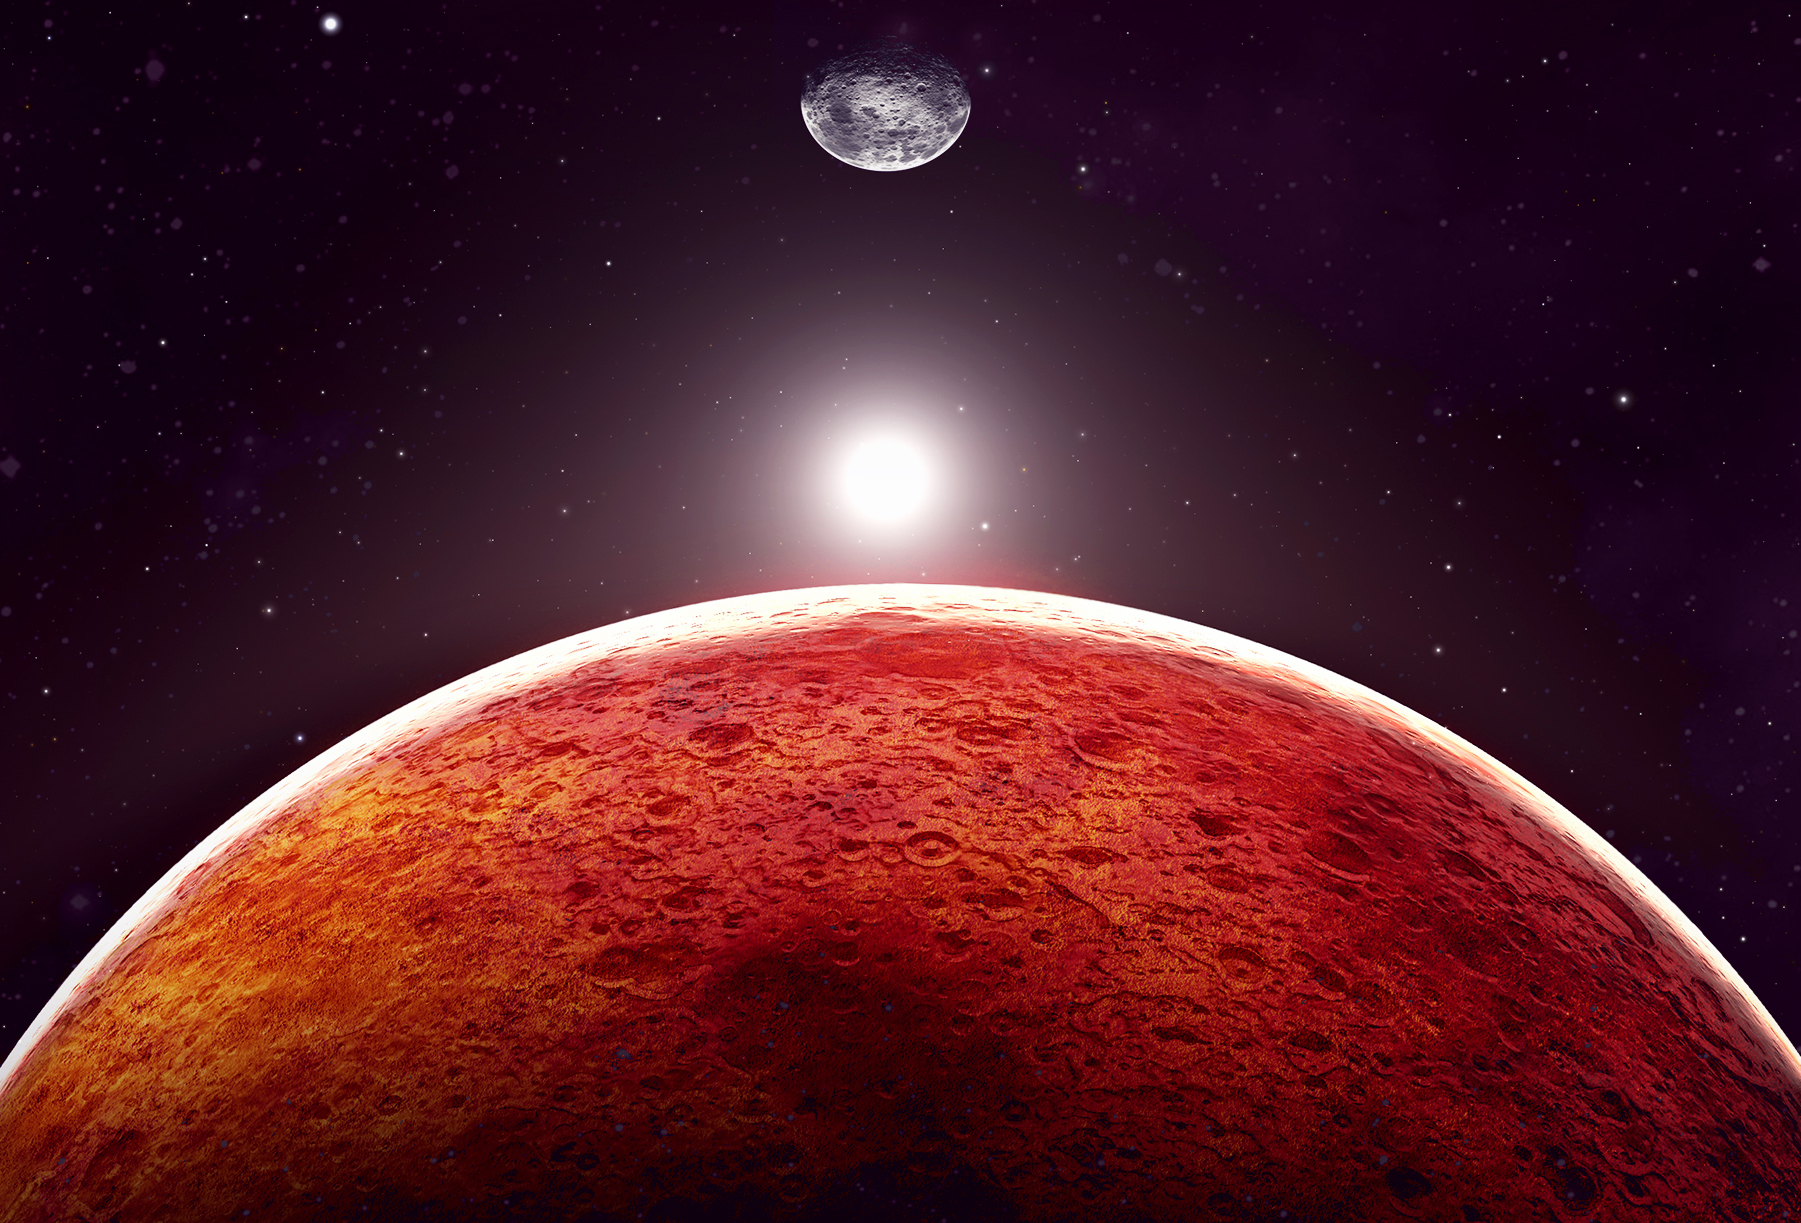
\includegraphics[width=0.80\textwidth, frame]{cover/MovingMarsfront_top}~\\[1cm]

% Title
\HRule \\[0.4cm]
{ \Huge \bfseries Moving Mars \\[0.4cm] }
\HRule \\[1.5cm]

% Author
\noindent
\begin{minipage}{0.4\textwidth}
\begin{center} \large
\emph{by}\\
David P. Hyland-Wood
\end{center}
\end{minipage}%

\vfill

% Bottom of the page
{\large \today}

\end{center}
\end{titlepage}

% General definitions for all Chapters
%-------------------------------------------------------------------------------
% Define Page style for all chapters
\pagestyle{fancy}
% Delete the current section for header and footer
\fancyhf{}
% Set custom header
\lhead[]{\thepage}
\rhead[\thepage]{}
% Set arabic (1,2,3...) page numbering
\pagenumbering{arabic}
% Set double spacing for the text
\doublespacing

% Frontmatter
%-------------------------------------------------------------------------------
\frontmatter
% Frontmatter "chapters" have no chapter numbers, so use '\chapter*'.

%%%%%%%%%%%%%%%%%%%%%%% dedication.tex %%%%%%%%%%%%%%%%%%%%%%%%%%
% 
% dedication
% 
%%%%%%%%%%%%%%%%%%%%%%%%%%%%%%%%%%%%%%%%%%%%%%%%%%%%%%%%%

\thispagestyle{empty}
\begin{dedication}
This book is dedicated to the children of the children who watched the Apollo missions with awe and hope.
\end{dedication}

% If the chapter ends in an odd page, you may want to skip having the page
%  number in the empty page
\newpage
\thispagestyle{empty}
%%%%%%%%%%%%%%%%%%%%%%preface.tex%%%%%%%%%%%%%%%%%%%%%%%%%%%
% 
% Acknowledgements
% 
%%%%%%%%%%%%%%%%%%%%%%%%%%%%%%%%%%%%%%%%%%%%%%%%%%%%%%%

\chapter*{Acknowledgements}

TODO, especially to acknowledge reviewers prior to publication and any contributors via GitHub.


% If the chapter ends in an odd page, you may want to skip having the page
%  number in the empty page
\newpage
\thispagestyle{empty}

%%%%%%%%%%%%%%%%%%%%%%preface.tex%%%%%%%%%%%%%%%%%%%%%%%%%%%
% 
% Preface
% 
%%%%%%%%%%%%%%%%%%%%%%%%%%%%%%%%%%%%%%%%%%%%%%%%%%%%%%%

\chapter*{Preface}
\addcontentsline{toc}{chapter}{Preface} % Add to TOC

Every book I have ever read has had typos, plot inconsistencies, mathematical errors, or conceptual errors. The best books keep these to a minimum, but they are still present. Can't we do better? The Internet should allow us to give feedback to authors and publishers, so they can fix their work, and make improvements.

Software developers have been doing this for a long time. GitHub is a site that allows many people to work on a single software project. In the case of Open Source Software, where the software is licensed for use by anyone, GitHub repositories of the source code may be copied (``forked'', in the parlance), modified by someone else, and the changes hopefully submitted to the original developers via a so-called ``pull request''. A contributor asks the original developers to ``pull'' his or her suggested changes into the project's source code.

This book is an experiment in collaborative writing. The book's source material is provided on GitHub, just like an Open Source Software project, and is licensed under the GNU Free Documentation License, Version 1.3. Anyone can fork the book into their own GitHub project, make suggestions for changes, and submit a pull request to me. If I accept some or all of your suggestions, I will add your name to the acknowledgements, and thank you publicly.

This book is hosted on GitHub at \url{https://github.com/prototypo/MovingMars}. I can also be reached via \url{https://hyland-wood.org}.

Come, let us write together.


% TODO: Typeset properly. Fredericksburg, Virginia, United States of America, June 2015


% If the chapter ends in an odd page, you may want to skip having the page
%  number in the empty page
\newpage
\thispagestyle{empty}

%%%%%%%%%%%%%%%%%%%%%%preface.tex%%%%%%%%%%%%%%%%%%%%%%%%%%%
% 
% Note to the Reader
% 
%%%%%%%%%%%%%%%%%%%%%%%%%%%%%%%%%%%%%%%%%%%%%%%%%%%%%%%

\chapter*{Note to the Reader}
\addcontentsline{toc}{chapter}{Note to the Reader} % Add to TOC

This is a work of speculative fiction. The world it describes is a puzzle. Some people enjoy working out the puzzle for themselves. If you prefer to do that, stop reading this note before you spoil the fun for yourself.

Others prefer to read without working out a puzzle. If that's you, then read on.

TODO: Pull in notes on world description, and terminology.


% If the chapter ends in an odd page, you may want to skip having the page
%  number in the empty page
\newpage
\thispagestyle{empty}


% Table of Contents
%-------------------------------------------------------------------------------
\newpage
% Use dots between chapter name and page number
\renewcommand{\cftchapdotsep}{\cftdotsep}
% Include the ToC
\tableofcontents

% If the chapter ends in an odd page, you may want to skip having the page
%  number in the empty page
\newpage
\thispagestyle{empty}

% Mainmatter
%-------------------------------------------------------------------------------
\mainmatter
% Mainmatter chapters have chapter numbers, so use '\chapter'.

% Chapter 1
%%%%%%%%%%%%%%%%%%%%%%%%%%%%%%%%%%%%%%%%%%%%%%%%%%
%
% Chapter:  Albatenius
%
%%%%%%%%%%%%%%%%%%%%%%%%%%%%%%%%%%%%%%%%%%%%%%%%%%

\chapter{Albatenius}

The spacecraft slept.

Its Italian builders had given it a short, Latinised name. That was probably called for, since the ninth century solar astronomer for which it was named, Ab\=u 'Abd All\={a}h Mu\d{h}ammad ibn J\={a}bir ibn Sin\={a}n al-Raqq\=\i{} al-\d{H}arr\={a}n\=\i{} a\d{s}-\d{S}\={a}bi' al-Batt\={a}n\=\i{}, did have a very long name. They called it, echoing their medieval ancestors, Albatenius.

Albatenius was well past its mission observing the Sun. Its solar arrays had been heavily bombarded by the stellar wind, the charged particles had damaged the silicon junctions that produced electrical power. Its batteries, after years of hysteresis, could no longer retain much electrical potential. The few sips of hydrazine remaining in its thruster tanks were frozen solid against the aluminium walls. Albatenius was little more than space junk, listing sideways, spinning slowly in the vacuum of space.

The spacecraft awoke.

Waking might be too strong a metaphor. A signal was received, processed, and responded to. No one had called in many years. But the radiation-hardened computer still operated, as did one of the radio transceivers. The batteries held enough power for some limited operation.

Current passed through copper traces etched onto its circuit boards. No motors were actuated, no motion was caused. But there was action. Inventory was taken. Status was checked. Slowly, carefully, always aware of the exact amount voltage drained from the aged batteries, Albatenius was stirred by an unseen hand.

No attempt was made to investigate the scientific instruments. They were hardly important now. The spacecraft had measured the ion and electron composition of the solar wind for an entire 7-year solar cycle. Other spacecraft had done the same. It was enough to guess what the flux would be at the first Lagrange point of the Earth-Sun system. L1 was a well-studied region of space.

The x-axis gyroscope was known to be frozen. The z-axis one, too. The operator didn't dare waste the few precious volts remaining in the batteries. There was no attempt to restore them. The remaining two gyroscopes were touched ever so gently in turn. A hint of voltage was applied to the y-axis gyroscope. Its sensors reported no movement. A pause. Finally, as if knowing the finality of the operation, another hint of voltage was applied to the off-axis gyroscope. Nothing. Another pause.

With nothing to lose, a stronger voltage tickled the off-axis gyroscope. A wiggle, so slight it could have almost been sensor noise, registered. There was a bit of life in the old girl yet. Another pause.

Full voltage was applied to the last gyroscope for a few seconds. The gyroscope rotated just enough to start the spacecraft spinning slowly. It took every last bit of the remaining battery power to spin the last gyroscope a few more precious seconds for an equal but opposite spin. Albatenius slowed to a halt, the same as it was with a tiny but important difference. Its damaged solar arrays now pointed more or less toward the Sun. The batteries began, slowly but inexorably, to charge.


% If the chapter ends in an odd page, you may want to skip having the page
%  number in the empty page
\newpage
\thispagestyle{empty}

% Chapter 2
%%%%%%%%%%%%%%%%%%%%%%%%%%%%%%%%%%%%%%%%%%%%%%%%%%
%
% Chapter:  Aapo
%
%%%%%%%%%%%%%%%%%%%%%%%%%%%%%%%%%%%%%%%%%%%%%%%%%%

\chapter{Aapo}

The priest arrived the day before my twelfth birthday. I didn't think they were supposed to do that.

Mum was scared. Her eyes widened when she opened the door from our room to the hall. Her head snapped back when she saw the yellow robes. She took a little half-step backward into my brother Thomas, and would have fallen over him if he hadn't put up his hands. Thom didn't move, though. He didn't want to chance missing the most exciting thing he had ever seen. Mum accidentally stepped hard on his foot, but he didn't say anything.

The priest stood at the door and waited. I suppose she was used to this reaction. At least that's how they always showed people reacting in the proms. Her long robes covered her from shoulders to a few centimetres above her sandals. Her hood was folded back so we could see her face. She was bald, of course, but you could see from her eyebrows that she was blonde. It was very hard to judge her age.

``Mrs. Filandros?'' she asked. Mum didn't move. ``Mrs. Filandros, I'm here to see your son Aapo.''

The priest seemed polite, even almost politely deferential. She didn't need to be, of course. She could have barged in, and taken what she wanted. We certainly couldn't have stopped her. But she seemed content to let events take their course.

``What did he do?'' Mum managed to squeak. She and Thom were still blocking the short hallway.

``All will become clear in time.'' Now that sounded like a priest. ``May I come in, please?''

Mum shooed Thom into our room. There was no place to hide him, and no time. In any case, the priest had seen him already. Thom slammed his shoulder into me. He tried to make it look like an accident. It wasn't, though. His face came up to my ear. ``Now you're going to get it. She's here for you.''

Our bedding was stored below the floor for the day. Dad was plugged in, so he hadn't noticed anything yet. Mum was pulling on his mask.

``Hey! Park-shi, my sincere apologies. My room seems crowded today. I assure you I am ready to serve y...'' Dad froze. ``Oh.'' The mask dropped on the floor. Mr. Park had a brief view of our ceiling before the connection severed.

``Mrs. Filandros, my name is Guang. Just relax.''

``Ni hao, laoshi.'' Mum stammered her heavily anglicised Chinese. At least she had recovered her manners.

``Isn't Guang a boy's name?" Thomas asked before Mum could stop him. He wasn't the best Mandarin student. He wasn't the best anything student. The only reason for a priest to be interested in him would be to assign him a task.

Guang looked at Thomas kindly. ``Only sometimes. Now, Mrs. Filandros, I'm here to speak with Aapo. Aapo, come with me.''

I stood up. I knew I couldn't risk looking at my parents. What had I done? Guang was no neighbourhood priest. Her robes were yellow, like a pulpiteer's, or the ones you saw on the proms in the big temples, the sanctuaries. I picked up my slate.

``No, leave it, please.''

I dropped the slate on a pillow, unused to being separated from it even when I was working on the farm. I followed her out into the hall, and could hear Mum crying. She had already figured out what the likely outcome of this was, then.

The priest went to the end of the building, down the two flights of stairs, and right into the vegetable gardens. We weaved through the beds for about a hundred meters, and then to the edge of the planted fields. In the old days, we might have grown corn, wheat, peas, or soybeans in the bare dirt. Our fields held trays stacked five deep held up by plastic poles. Each top tray held a type of hydrogenotrophic bacteria that made amino acids, and then proteins. The three middle ones were sealed, and partially pressurised, to make edible, burnable, and lubricating oils from similar types of bacteria. The bottom ones held yeasts that our outlying kitchens would use to make breads.

Eventually we came to a small, unplanted rise with a bench on it. The Stebling twins were already there. They jumped up at the unexpected sight of a priest. We took ownership of the bench as they ran to tell the news to the rest of the dunbar.

``Aapo, what is the integral of e\textsuperscript{x} with respect to x?''

``e to the x plus a constant, laoshi.''

Guang smiled and shook her head. ``Hah. Nearly everyone forgets the constant. All right, why do we care about the calculus?''

``Do you mean the infinitesimal calculus, laoshi?'' I asked.

``Yes.'' She paused. ``How many other calculi do you know?''

``I know the propositional calculus, and the lambda calculus. I have only just started the process calculus.''

``That's fine. So why do we care about the infinitesimal calculus?''

``It is used to describe changing systems, laoshi.''

``Can you name a few systems that change?''

I thought for a moment. ``I can't think of any systems that don't change, laoshi.''

``What about purely theoretical systems?''

``Sure, but no one seems quite certain that they really exist. I think they might just be patterns of heavy weighting in our neocortex.''

``Hmm. Perhaps. Let's leave epistemology for now. Let's say that I will take you to the sanctuary if you are good at maths, and I will take you back home if you are not. Clearly you are either good at maths or you are not. Without knowing which is the case, what do you know from those statements?''

``I know that you will either take me to the sanctuary or back home.''

``And how do you know that?''

``It is a destructive dilemma, a type of inference, laoshi.''

Guang sat quietly. She seemed lost in thought. The wind ruffled the sleeves of her robes. A mosquito landed on her left ear. Its proboscis worked its way into the very top of the auricle. If she noticed, she didn't seem to care. Her eyes became focused on the towers of a milk processing plant on a ridge to our south, part of another dunbar. Minutes passed.

I fidgeted. I reached for my slate, then realised with a start that I didn't have it. I looked at my sandals, at the worn leather of the straps, then at my fraying pant legs. I started to kick my feet back and forth in the air, then self consciously stopped.

I tried to wait. Failing, I looked again at the eerily still priest. I could now see the fine wrinkles around her eyes in the sunlight, and revised her age upward. She might have been in her forties, like Mr. and Mrs. Stebling. She was younger than my parents, I thought, then thought again. My parents worked outside in the fields. Maybe she was older than them after all. Maybe she stayed inside more.

Her eyes refocused on me. ``Can you think of an algorithm that takes two lambda expressions and returns a boolean indicating whether the two expressions are computationally equivalent to one another?''

``No, laoshi. Nobody can. Such equivalence is undecidable.''

``Very well. We can go speak with your parents now.''

With relief, I followed Guang back through the vegetable beds, and up the front steps into our building. Our dunbar wasn't rich, but it wasn't poor either. Our front hall had a reasonable number of awards for productivity from the local temple. Our History hung on the wall opposite the front door, pictures of generations past that had built the building and the farm. We could easily feed ourselves and all the others who operated factories in the surrounding hills. From the top of the steps you could see the fields spreading out around us with their stacked trays.

We might not be rich, but we could take pride in the work we did. It was useful work. That's what Elder Mattias and our old people said. But it was boring work. I preferred the games on my slate.

We walked through our front hall, and turned right toward the stairs we had come down. Our communal kitchen was on our left, and the dining hall on our right. The other side of our building held our meeting house. I could see Isabella Stebling talking animatedly to Mrs. Reynolds and old Mr. Wu in the kitchen. Her sister Sophia pointed to me as we passed. She was careful to make sure Guang didn't see her.

My parents hadn't closed the door to our room. Elder Mattias, our neighbourhood priest, was standing by our door in the taupe robes of a retiree, his bald head gleaming a bit in the reflected light from the hallway fixtures. He was the oldest person I knew. There were rumours that he was well over 100. He had been with us for most of my life, and all the years I had memories. Of course, he was still an outsider to the members of our close-knit dunbar. He always would be. He just wasn't born here.

Mum and Dad were sitting on the tatami, not moving at all. Mum looked unwell, but at least she had stopped crying. Dad was holding her hand.

``Mr. and Mrs. Filandros, I am going to take Aapo with me. He will be able to communicate with you after he settles into the sanctuary.'' Guang waited while the shocked silence passed.

``But\ldots{} the sanctuary. Why? Are you sure you have the right child? Aapo is a good boy, but he is not much of a student. He isn't even a hard worker. He mostly sits and plays games.'' My Dad took the lead since Mum was seemingly incapable of speech.

``Yes, but it is Aapo's progress in a particular game we are interested in.''

``What do you mean? Po, which game have you spent so much time on?''

Mum didn't seem to be present in the small room. She resumed crying quietly, lost in her own thoughts. Her hands covered her face, her hair covering her hands. I realised that Dad had asked me a question, and was looking at me.

``It's called Curveball, Dad.'' I said. ``You need to manoeuvre a ball across a landscape described by some equations. It starts really easy, like with a circle, then an infinite plane. Then it gets harder. By the time you hit the upper levels you need to really think about the problems before you give an answer. Sometimes it takes me a few days to figure one out.''

``Curveball?'' asked Thomas. ``I've played Curveball. I'm pretty good at it.'' Mum's head snapped up at this. She stared at Thom like he had just admitted to a murder.

``How many levels have you completed, Thomas?'' asked Guang.

``Twenty four.'' Thom answered proudly.

``Your younger brother is on level two hundred and thirty one.''

``Two hundred and thirty one?? That's not possible. Each level is a lot harder than the one before!''

``That's right. The first hundred are, in fact, exponentially harder. Aapo is well into temple-level mathematics.''

``He's not even twelve, laoshi. How can this be?'' Dad asked.

``Apparently,'' Guang said patiently, ``he is good at it.'' She waited serenely. Minutes passed. There were no more questions.

I started into my room to get my clothes. Elder Mattias blocked my way. ``You already have everything you need, Po.''

I looked to Guang. ``You will be given new clothes at the sanctuary.'' I realised that I didn't have my slate. Was I really to be separated from it? The thought made me slightly ill. I couldn't ask her, though. One did not demand things from yellow-robed priests.

Dad stared at her, then at Thom, then at me. He chewed his lip. ``What will happen to him?'' he blurted.

Guang turned, and headed back toward the stairs. Elder Mattias stayed at his station in the doorway. The message was clear. I exchanged glances with my parents for the last time before skipping to catch up with her. She didn't seem to notice my momentary lagging. At least she didn't berate me for it.

``Please, what will happen to him?'' I heard my dad ask again, his voice fading as we moved farther down the hallway.

Mrs. Reynolds, her husband Jacob, twenty or thirty others of the closest friends I would ever have were all staring silently at us as we walked through the front hall. Isabella was holding a dandelion blossom, and looked like she wanted to give it to me. She didn't have the chance. Mr. Wu, who had bounced me on his knee when he was only in his seventies, laid his hand on my head for a moment. I was too numb to ask them to say goodbye to everyone else. I could see some of the younger children fanning out through the fields to tell the rest of my dunbar. The occasional head craned upward, looking over the crops.

We walked out of the only world I had ever known.


% If the chapter ends in an odd page, you may want to skip having the page
%  number in the empty page
\newpage
\thispagestyle{empty}

% Chapter 3
%%%%%%%%%%%%%%%%%%%%%%%%%%%%%%%%%%%%%%%%%%%%%%%%%%
%
% Chapter:  Underway
%
%%%%%%%%%%%%%%%%%%%%%%%%%%%%%%%%%%%%%%%%%%%%%%%%%%

\chapter{Underway}

The spacecraft awoke.

Albatenius received a new command, and unthinkingly executed it. The batteries had stopped taking a charge from the solar panels. No more electrical potential could be acquired. It would have to be enough.

The two wings of solar panels twisted to make their angle almost parallel to the Sun's rays. Two slight nudges from the remaining gyroscope twisted the spacecraft farther around. The thin solar wind would impact the spacecraft just a bit less. It, too, would have to be enough.

No spacecraft could sit forever in an L1 point, where the Sun's and Earth's gravity were felt in equal amounts. Staying exactly in L1 was like sitting on the top of a long pole. The slightest wavering in one direction or another would cause the gravitational tug of either the Sun or the Earth to dominate. So spacecraft orbited the point in a so-called halo orbit, circling around L1 as if it were itself a gravity well.

Albatenius' solar panels moved again, back to face the Sun. A quarter of an orbit later, they moved perpendicular again. And so it went. Back and forth, each movement changing the tiny force of the solar wind. Days passed, then weeks. The tiny halo orbit began to weaken, to elongate. Finally, it broke. Albatenius sailed free of the L1 point, and slowly into a highly elliptical orbit around Earth.

Another command realigned the solar panels to charge the batteries back to their full potential. Another waiting game ensued. Coaxing a nearly dead spacecraft into travel was a subtle game, full of careful consideration, careful timing, and even more careful use of scarce resources.

Two hundred and three Earth orbits later, having miraculously missed each of the spacecraft in low Earth orbit and most of the space junk in its perigee, Albatenius felt the gravity of a near-Earth asteroid. The asteroid TODO...

TODO: describe a horseshoe orbit here, and have the asteroid throw the spacecraft out of Earth orbit toward the asteroid belt.

% If the chapter ends in an odd page, you may want to skip having the page
%  number in the empty page
\newpage
\thispagestyle{empty}

% Chapter 4
%%%%%%%%%%%%%%%%%%%%%%%%%%%%%%%%%%%%%%%%%%%%%%%%%%
%
% Chapter:  First Rock
%
%%%%%%%%%%%%%%%%%%%%%%%%%%%%%%%%%%%%%%%%%%%%%%%%%%

\chapter{First Rock}

Two hundred and three Earth orbits later, having miraculously missed each of the spacecraft in low Earth orbit and most of the space junk at its perigee, Albatenius felt the gravity of a near-Earth asteroid. The asteroid's pull was ever so subtle, but it was importantly, critically present.

Another few hundred orbits. Silent, waiting, being.

The NEO didn't just pull on Albatenius. The spacecraft also pulled back, so slightly it could only be noticed over a very long timeframe. Naively, it was a classic three-body problem of spacecraft, rock and Earth. In reality, it was far more complex due to all the other small bodies scattered near their orbits. It was certainly nondeterministic over a long enough period. There was no way to tell what would happen. But one could observe and, eventually, carefully, react.


% If the chapter ends in an odd page, you may want to skip having the page
%  number in the empty page
\newpage
\thispagestyle{empty}


% Backmatter
%-------------------------------------------------------------------------------

% Backmatter "chapters" have no chapter numbers, so use '\chapter*'.

%%%%%%%%%%%%%%%%%%%%%%% acknowledgements.tex %%%%%%%%%%%%%%%%%%%%
% 
% About the Author
% 
%%%%%%%%%%%%%%%%%%%%%%%%%%%%%%%%%%%%%%%%%%%%%%%%%%%%%%%%

%\chapter*{About the Author}
\vspace*{\fill}
\begin{center}
\section*{\textbf{About the Author}}
\end{center}
\addcontentsline{toc}{chapter}{About the Author} % Add to TOC


Dr. David Hyland-Wood has been a ship navigator, deep sea salvage engineer, aerospace engineer, university researcher, lecturer, and software entrepreneur. David holds university degrees in mechanical, aeronautical, astronautical, and software engineering. He lives in Mission Beach, Australia. This is his first work of fiction.

David may be reached via \href{hyland-wood.org}{hyland-wood.org}.
\vspace*{\fill}
% Added to TOC in the chapter file

\clearpage
\addcontentsline{toc}{chapter}{Index} % Add to TOC
\printindex
%-------------------------------------------------------------------------------

\end{document}

